\documentclass[10pt,twocolumn]{article}
\usepackage[margin=0.64in,columnsep=0.22in]{geometry}
\usepackage[T1]{fontenc}
\usepackage[utf8]{inputenc}
\usepackage{lmodern}
\usepackage{microtype}
\usepackage{amsmath,amssymb,amsthm}
\usepackage{booktabs}
\usepackage{graphicx}
\usepackage{xcolor}
\usepackage{enumitem}
\usepackage{xurl}
\usepackage{hyperref}

\hypersetup{
  colorlinks=true,
  linkcolor=blue!60!black,
  citecolor=blue!60!black,
  urlcolor=blue!60!black,
  pdftitle={Constructive Lean 4 Formalization and Exact-Rational Certificates for Polynomial-Time 1/5-Approximate Nash Equilibria},
  pdfauthor={Lluis Eriksson}
}

\newtheorem{proposition}{Proposition}
\newtheorem{definition}{Definition}
\newcommand{\QQ}{\mathbb{Q}}
\newcommand{\ZZ}{\mathbb{Z}}

\title{\vspace{-1.0em}\textbf{Constructive Lean~4 Formalization and Exact-Rational Certificates for Polynomial-Time $1/5$-Approximate Nash Equilibria}}
\author{Lluis Eriksson\thanks{Independent Researcher. Code, Lean~4 proofs, and certificates: MIT License; manuscript and figures: CC-BY-4.0. Prepared with transparent AI coding, formalization, and drafting assistance via Google Antigravity; all Lean~4 theorems, exact-$\QQ$ verifiers, and adversarial tests were independently compiled and verified locally. Repository: \href{https://github.com/lluiseriksson/cogentic-maximin-kite-nash-certificates}{\nolinkurl{github.com/lluiseriksson/cogentic-maximin-kite-nash-certificates}}.}}
\date{November 25, 2026}

\begin{document}
\maketitle
\vspace{-1.3em}

\begin{abstract}
Google Research Cogentic (Nov.~25, 2026) introduced \texttt{MaximinKiteNE}, a deterministic polynomial-time algorithm computing an exact rational $1/5$-approximate Nash equilibrium ($\delta = 0$) in any $[0,1]$-normalized rational bimatrix game, breaking the $1/3+\delta$ barrier. Because that preprint is accompanied by neither machine-checked formalizations nor executable exact-rational verifiers and the halting proof rests on a delicate chain of exact rational inequalities—from $s$-kite best-response mixing and the $7/4$ welfare cap to the Stage~4 functional bound $H(z,c_1,c_2) \le -1/3000 < -2^{-14}$—independent formal verification is essential. We deliver an open, zero-dependency, zero-floating-point verification stack pairing: (i)~\texttt{MaximinKiteNash.lean}, 18 constructive Lean~4.35.0 theorems (zero \texttt{sorry}, zero \texttt{axiom}, zero \texttt{Classical.choice}, kernel axioms strictly \texttt{[propext, Quot.sound]}) mechanizing the deterministic algebraic, primal-dual, simplex-rounding, square-completion, shifted-cubic, and contradiction pillars; and (ii)~\texttt{KITE-NASH-CERT-1.0}, a pure-stdlib Python \texttt{fractions.Fraction} auditor across four modes. We certify 16 canonical witnesses in $0.104$--$2.564\,\mathrm{ms}$, independently verify $H(z,c_1,c_2) \le -1/1280 \le -1/3000$ across a $13^3 = 2{,}197$-point exact rational grid on $[1/4,4]^3$, reject 60/60 live adversarial forgeries plus raw IEEE-754/\texttt{NaN}/duplicate-key tokens, and enforce a 40-file SHA-256 manifest.
\end{abstract}

\section{Introduction and Scope Calibration}\label{sec:intro}
Computing an $\varepsilon$-approximate Nash equilibrium ($\varepsilon$-NE) in a two-player bimatrix game $(R,C) \in ([0,1]\cap\QQ)^{m\times n}$ has progressed from $\varepsilon=1/2$~\cite{daskalakis2006note}, $(3-\sqrt{5})/2 \approx 0.38197$~\cite{daskalakis2007progress}, $0.36392$~\cite{bosse2007new}, and $0.3393$~\cite{tsaknakis2008optimization} to $1/3+\delta$~\cite{deligkas2022gradient}. On November~25, 2026, Google Research Cogentic~\cite{cogentic2026maximin} presented \texttt{MaximinKiteNE}, achieving exact polynomial-time $1/5$-NE ($\delta=0$) via four stages: (1)~exact zero-sum minimax screening $(v_R,v_C)$; (2)~primal-dual $1/5$-kite queries anchored at weight $1/4$ to $x_{\mathrm{mm}}$ across a $K_1 = 3\cdot 256 = 768$-scale discrete filter bank; (3)~continuous-time Volterra interpolation and Plancherel/FTC scale-lag estimates forcing $H(z,c_1,c_2) \ge -2^{-14}$ on $[1/4,4]^3$ if the loop never halts; and (4)~exact rational algebraic certification proving $H(z,c_1,c_2) \le -1/3000 < -2^{-14}$ everywhere on $[1/4,4]^3$.

\paragraph{Honest Two-Layer Verification Scope.}
We strictly separate what is machine-checked from what remains external to our Lean kernel:
\begin{enumerate}[leftmargin=1.3em,itemsep=1pt,topsep=2pt]
  \item \textbf{Layer~1 (Lean~4.35.0 Kernel, Universal Algebraic \& Structural Pillars):} \texttt{MaximinKiteNash.lean} proves 18 zero-dependency integer and inductive-list theorems (Table~\ref{tab:lean18}) covering Lem.~2.3(a)--(b) $s$-kite mixing, the $7/4$ welfare cap, Lem.~2.2 minimax regret screening, weak duality, dual weight ratio $a\in[1/4,4]$, Lem.~2.1(b) simplex rounding $L_1$/remainder bounds, $1/4$-maximin anchoring, Sec.~2.3 step-parameter arithmetic, Lem.~5.2 Eq.~(5.7) square completion, Lem.~5.1(3) Eq.~(5.3) shifted-cubic identity, Subcase~1(b) universal discriminant polynomial identity, Eq.~(5.8) margin $-613/97280 < -1/3000$, Sec.~5.3 high-gate breakpoint ordering, and $-1/3000 < -2^{-14}$.
  \item \textbf{Layer~2 (Exact-$\QQ$ Certificate Auditor):} \texttt{KITE-NASH-CERT-1.0} replays concrete finite bimatrix games, minimax saddle points, simplex roundings, and exact Stage~4 $H(z,c_1,c_2)$ evaluations over $\QQ$ without floating-point arithmetic.
  \item \textbf{Explicit Non-Claims:} We do \emph{not} formalize strong LP duality, polynomial-time ellipsoid/interior-point solvers, the continuous-time Volterra interpolation, Plancherel's theorem, or the full continuum cell-cover proof of Lemmas~5.2--5.4 inside Lean~4; those analytical steps remain in~\cite{cogentic2026maximin}.
\end{enumerate}

\section{Exact Stage~4 Rational Functional}\label{sec:stage4}
To guarantee self-contained auditability solely from this manuscript, we record the exact piecewise-rational formulas of~\cite{cogentic2026maximin} (Eqs.~(4.1)--(4.8) and Lem.~5.1(1)) implemented verbatim in \texttt{src/kite\_exact.py}. For $(z,c_1,c_2)\in[1/4,4]^3$ and $u_+ := \max(u,0)$:
\begin{align}
f(z) &:= \begin{cases} 1, & z\in[\tfrac14,1],\\ \tfrac{4z+1}{5}, & z\in(1,2],\\ \tfrac95, & z\in(2,4], \end{cases}\label{eq:gate}\\
\lambda_K(z,y) &:= \tfrac{f(z)}{128}\min\!\big(1,8(z{-}\tfrac78)_+\big)\nonumber\\
&\quad \times\big(1+\min(1,4(y{-}z)_+)\big),\nonumber\\
\Lambda(z,y) &:= \tfrac{f(z)}{8} + \tfrac{3(y+f(z)z)+(y+f(z)z-2f(z))_+}{32}\nonumber\\
&\quad + \tfrac{4(y-f(z)z)_+}{32} - \tfrac{(y-z)_+}{8} - \tfrac{f(z)z}{5} + \lambda_K(z,y).\label{eq:Lambda}
\end{align}
Writing $f_0 = f(z)$, $A := (c_2+f_0 c_1-2f_0)/2$, and $B := (c_2-f_0 c_1)/2$, the closed-form integral $J(f_0;c_1,c_2)$ and its piecewise-linear envelope $J_{\mathrm{mid}}$ satisfy $J \le J_{\mathrm{mid}}$ (Prop.~4.1(1)) with equality whenever $AB \ge 0$:
\begin{equation}
J(f_0;c_1,c_2) = \begin{cases}
0, & A\le 0,\,B\le 0,\\
\frac{c_2-f_0}{16}, & A\ge 0,\,B\ge 0,\\
\frac{(c_2+f_0 c_1-2f_0)^2}{64 f_0(c_1-1)}, & A>0>B,\\
\frac{(c_2-f_0 c_1)^2}{64 f_0(1-c_1)}, & A<0<B,
\end{cases}\label{eq:J}
\end{equation}
$J_{\mathrm{mid}} := \frac{(c_2+f_0 c_1-2f_0)_+ + 2(c_2-f_0)_+ + (c_2-f_0 c_1)_+}{64}$, and
\begin{align}
F(f_0;c_1,c_2) &:= \tfrac{f_0 c_1 - c_2}{8} + \tfrac{3(c_2+f_0 c_1)^2 + (c_2+f_0 c_1-2f_0)_+^2}{64 f_0}\nonumber\\
&\quad - \tfrac{4(c_2-f_0 c_1)_+^2}{64 f_0} + J + \tfrac{(c_2-c_1)_+^2}{16} - \tfrac{f_0 c_1^2 + c_2^2}{10}.\label{eq:F}
\end{align}
Finally, with variance term $E_{\mathrm{var}}(z;c_1,c_2)$ equal to $\min\big(\frac{5}{1536}, \frac{5}{162}(\frac{c_1+c_2}{2}-\frac14)_+^3\big)$ when $z\le\frac34$ and $c_1+c_2\le 2$, equal to $\frac{5}{1536}$ on the rest of $z\le\frac78$, and $\frac{5 f(z)}{6144}$ for $z>\frac78$, the Stage~4 functional is
\begin{align}
H(z,c_1,c_2) &:= F(f_0;c_1,c_2) - \Lambda(z,c_2)(c_1-z)\nonumber\\
&\quad - \Big(\tfrac18 - \tfrac{c_2}{80}\Big)(z-c_2) + E_{\mathrm{var}}.\label{eq:H}
\end{align}
Replacing $J$ by $J_{\mathrm{mid}}$ yields the Lemma~5.1(2) upper bound $H_{\mathrm{up}} = G_{\mathrm{mid}}(z,c_2) + h_{\mathrm{comb}}(c_1) + E_{\mathrm{var}} \ge H$.

\section{Constructive Lean~4.35.0 Kernel}\label{sec:lean}
\texttt{lean/MaximinKiteNash.lean} compiles standalone in $3.2\,\mathrm{s}$ under Lean~4.35.0~\cite{demoura2021lean4} with zero Mathlib or external imports. Table~\ref{tab:lean18} lists the exact formalized statement of every theorem.

\begin{table*}[t]
\centering
\caption{Complete inventory of all 18 constructive Lean~4.35.0 theorems in \texttt{lean/MaximinKiteNash.lean} (zero \texttt{sorry}, zero \texttt{axiom}, zero \texttt{Classical.choice}; every theorem audits strictly to \texttt{[propext, Quot.sound]} via \texttt{lake env lean -j 1 AuditAxioms.lean}).}
\label{tab:lean18}
\scriptsize
\setlength{\tabcolsep}{3.0pt}
\begin{tabular}{@{}r l l p{10.5cm}@{}}
\toprule
\# & Theorem Identifier & Ref.~\cite{cogentic2026maximin} & Exact Machine-Checked Statement (Cleared Integers / Inductive Lists) \\
\midrule
1 & \texttt{kite\_best\_response\_mixing\_row} & Lem.~2.3(a) & $s r_2 + (r_1{-}s)D \le s r_1 \iff (D{-}s)r_1 + s r_2 \le s D$ ($\forall D,s,r_1,r_2\in\ZZ$). \\
2 & \texttt{kite\_best\_response\_mixing\_col} & Lem.~2.3(a) & $s r_1 + (r_2{-}s)D \le s r_2 \iff s r_1 + (D{-}s)r_2 \le s D$ ($\forall D,s,r_1,r_2\in\ZZ$). \\
3 & \texttt{kite\_escape\_welfare\_cap\_general} & Lem.~2.3(b) & $2r<D,\,X,Y\le D$ and escaping either $r$-kite face $\implies (D{-}r)(X{+}Y) < D(2D{-}3r)$. \\
4 & \texttt{kite\_one\_fifth\_welfare\_cap\_7\_4} & Sec.~1.3 & $X,Y\le D$ and $4(D{-}X)+(D{-}Y)>D$ (or symm.) $\implies 4(X{+}Y) < 7D$. \\
5 & \texttt{zero\_sum\_minimax\_regret\_screen} & Lem.~2.2 & $0\le u_R,u_C$, $M_1\le v_R\le s$, $M_2\le v_C\le s \implies M_1{-}u_R\le s \wedge M_2{-}u_C\le s$. \\
6 & \texttt{zero\_sum\_weak\_duality\_sum} & Lem.~2.2/2.3 & Inductive list theorem: $\forall xs:\mathrm{List}(\ZZ{\times}\ZZ),\ \mathrm{AllNonnegPairs}(xs) \implies 0 \le \mathrm{dotInt}(xs)$. \\
7 & \texttt{kite\_dual\_lambda\_bounds} & Lem.~2.3(b) & $2r<D$, $t_1,t_2\ge 0$, $t_1+t_2=D \implies rD \le r t_1 + (D{-}r)t_2 \le (D{-}r)D$. \\
8 & \texttt{dual\_weight\_ratio\_range\_1\_4\_to\_4} & Sec.~1.3 & $D\le 5\lambda \le 4D \implies D{-}\lambda \le 4\lambda \wedge \lambda \le 4(D{-}\lambda)$ (i.e.\ $a=\frac{\lambda}{1-\lambda}\in[\frac14,4]$). \\
9 & \texttt{simplex\_rounding\_l1\_error\_bound} & Lem.~2.1(b) & Inductive list theorem: $\forall es:\mathrm{List}\,\ZZ,\ \mathrm{AllLe}(\mathrm{step},es)\implies \mathrm{sumList}(es)\le |es|\cdot\mathrm{step}$. \\
10 & \texttt{simplex\_rounding\_remainder\_bounds} & Lem.~2.1(b) & Inductive list theorem: $S>0,\,\mathrm{AllInRange}(S,fs)\implies 0\le \mathrm{sumList}(fs)$ and ($fs\ne [] \implies \mathrm{sumList}(fs)<|fs|\cdot S$). \\
11 & \texttt{anchored\_query\_convex\_combination} & Sec.~2.3 & $s_{\mathrm{MM}}=D,\,s_{\mathrm{Bar}}=D,\,5v_R>D \implies s_{\mathrm{MM}}+3 s_{\mathrm{Bar}}=4D \wedge 20 v_R > 4D$. \\
12 & \texttt{stage2\_universal\_step\_parameters} & Sec.~2.3 & $0<S_1,\varepsilon^{-1}$, $T_1=40 S_1\varepsilon^{-1}{+}1 \implies 0<T_1 \wedge 40 S_1\varepsilon^{-1}<T_1 \wedge 3\cdot 256=768 \wedge 2^{24}=16777216$. \\
13 & \texttt{stage4\_low\_gate\_square\_completion\_5\_7} & Eq.~(5.7) & $21(17(z{-}c_2)^2 + 4 c_2^2) = (21 c_2{-}17 z)^2 + 68 z^2 \ge 68 z^2$ ($\forall z,c_2\in\ZZ$). \\
14 & \texttt{stage4\_cubic\_Q\_bound\_eq5\_3} & Eq.~(5.3) & $27 Q((4{+}u)/3) = -36 - 60u - 219u^2 - 60u^3$ ($\forall u\in\ZZ$) and $28\cdot 477 = 13356 < 13400 = 536\cdot 25$. \\
15 & \texttt{stage4\_subcase1b\_discriminant\_negative} & Lem.~5.2 & $\forall s,D\in\ZZ,\ 204(16(D{-}s)^2{-}D^2)-14(10D{-}17s)^2 = 2(830 D^2{-}884 Ds{-}391 s^2)$; at $\frac{10}{17}$ equals $\frac{2970}{119}>0$. \\
16 & \texttt{stage4\_subcase1c\_margin\_eq5\_8} & Eq.~(5.8) & $5\cdot 95 - 17\cdot 64 = -613$, $1024\cdot 95 = 1520\cdot 64 = 97280 < 613\cdot 3000$ ($-\frac{613}{97280} < -\frac{1}{3000}$). \\
17 & \texttt{stage4\_high\_gate\_breakpoints\_order} & Sec.~5.3 & $D\le z\le 2D \implies f_0(2{-}z)\le f_0 \le z \le f_0 z$ (all 4 cleared-integer inequalities for $f_0=\frac{4z+D}{5D}$). \\
18 & \texttt{stage4\_final\_contradiction\_3000\_vs\_16384} & Thm.~5.5 & $2^{14}=16384>3000$ ($-\frac{1}{3000}<-2^{-14}$) and exact chain $\frac15 < \frac13 < \frac{3393}{10000} < \frac{3639}{10000} < \frac{3819}{10000} < \frac{3-\sqrt{5}}{2} < \frac12$ (via $5\cdot 10^8<22362^2$ and $2^2<5$). \\
\bottomrule
\end{tabular}
\end{table*}

\begin{proposition}[Machine-Checked Kernel Soundness]\label{prop:lean}
\normalfont Every theorem in Table~\ref{tab:lean18} compiles under Lean~4.35.0 without external dependencies, \texttt{sorry}, custom \texttt{axiom} declarations, or \texttt{Classical.choice}. In particular: (1)~Theorems~1--4 and~7--8 certify the exact $s$-kite dichotomy (in-kite mixing to exact $s$-NE vs.\ escaped welfare cap $X+Y < 7/4$ and dual weight ratio $a\in[1/4,4]$ at $s=1/5$); (2)~Theorems~5--6 and~9--11 certify the minimax regret screen, weak duality, denominator-$D$ simplex rounding $L_1$ and remainder bounds, and $1/4$-maximin anchoring; and (3)~Theorems~12--18 certify the Sec.~2.3 step-parameter arithmetic and the core Stage~4 rational algebraic identities forcing $-1/3000 < -2^{-14}$.
\end{proposition}

\section{Exact-\texorpdfstring{$\QQ$}{Q} Auditor \texorpdfstring{\texttt{KITE-NASH-CERT-1.0}}{KITE-NASH-CERT-1.0}}\label{sec:certifier}
\texttt{src/kite\_exact.py} and \texttt{src/kite\_certifier.py} use exclusively Python \texttt{int} and \texttt{fractions.Fraction}, statically checked by \texttt{scripts/verify\_all.py} for zero occurrences of \texttt{float(}, \texttt{math.}, \texttt{numpy}, or \texttt{np.}. Raw JSON parsing uses \texttt{parse\_float}, \texttt{parse\_constant}, and \texttt{object\_pairs\_hook} rejecting all decimal literals, \texttt{NaN}/\texttt{Infinity}, and duplicate object keys, followed by a strict AST type whitelist, nesting-depth cap ($20$), ASCII-digit canonical lowest-terms rational parsing (\texttt{len $\le 2000$}, rejecting leading zeros, \texttt{-0}, \texttt{+}, and unreduced fractions), and duplicate probe rejection.

\begin{definition}[\texttt{KITE-NASH-CERT-1.0} Acceptance Predicates]\label{def:cert}
\normalfont A JSON witness with \texttt{schema="KITE-NASH-CERT-1.0"} is accepted iff all claimed exact rational/integer summaries match recomputed values and its mode predicate holds:
\begin{itemize}[leftmargin=1.2em,itemsep=1pt,topsep=2pt]
  \item \textbf{Mode~1 (\texttt{kite\_best\_response\_and\_welfare\_cert}):} Given $s\in(0,1/2)$, $R,C\in([0,1]\cap\QQ)^{m\times n}$, and $x\in\Delta_m, y\in\Delta_n$, computes exact $(u_R,u_C,r_1,r_2)$. In \texttt{in\_kite}, enforces $(1{-}s)r_1+sr_2\le s$, $sr_1+(1{-}s)r_2\le s$, exact Lem.~2.3(a) mixing $(x_{\mathrm{out}},y_{\mathrm{out}})$ via verified pure best-response index, and $\max(r_1',r_2')\le s$. In \texttt{escaped\_welfare\_cap}, enforces escape of at least one kite face, strict cap $u_R+u_C < 2 - s/(1-s)$, dual multipliers $\theta_1,\theta_2\ge 0$ ($\theta_1+\theta_2=1$) satisfying Cogentic's Lem.~2.3(b) dual separation $\theta_1((1{-}s)r_1+sr_2) + \theta_2(sr_1+(1{-}s)r_2) = (1{-}\lambda^*)r_1+\lambda^* r_2 > s$, $\lambda^*=s\theta_1+(1{-}s)\theta_2\in[s,1{-}s]$, and $a=\lambda^*/(1{-}\lambda^*)\in[s/(1{-}s),(1{-}s)/s]$.
  \item \textbf{Mode~2 (\texttt{minimax\_screen\_and\_rounding\_cert}):} Verifies exact zero-sum saddle points $\min_j(x_{\mathrm{mm}}^T R)_j \ge v_R \ge \max_i(R y_{\mathrm{mm}})_i$ and $\min_i(C y_{\mathrm{col}})_i \ge v_C \ge \max_j(x_{\mathrm{guard}}^T C)_j$; checks denominator-$D$ simplex rounding $c_k\in\{\lfloor D p_k\rfloor,\lfloor D p_k\rfloor+1\}$, $\sum c_k=D$, $r=D-\sum\lfloor D p_k\rfloor\in\{0,\dots,d-1\}$, and $\|\hat{p}-p\|_1\le d/D$; enforces either \texttt{early\_halt} ($\max(v_R,v_C)\le s$, i.e., $v_R\le s \wedge v_C\le s$, with exact Lem.~2.2 minimax profile $(\text{halt\_x},\text{halt\_y})=(x_{\mathrm{guard}},y_{\mathrm{mm}})$ having regret $\le s$) or \texttt{anchored\_continue} (Row-oriented after Step~2: $v_R>s \wedge v_R\ge v_C$, $\tilde{x}=\frac14 x_{\mathrm{mm}}+\frac34\bar{x}$, and $\min_j(\tilde{x}^T R)_j \ge v_R/4 > s/4$).
  \item \textbf{Mode~3 (\texttt{stage4\_H\_algebraic\_cert}):} For a non-empty, duplicate-free list of triples $(z,c_1,c_2)\in[1/4,4]^3$ obeying the declared regime (\texttt{low\_gate\_z\_le\_1}, \texttt{high\_gate\_mid\_1\_to\_2}, \texttt{high\_gate\_top\_2\_to\_4}, or \texttt{mixed\_cube}), evaluates Eqs.~(\ref{eq:gate})--(\ref{eq:H}) exactly in $\QQ$ and checks: (i)~$J\le J_{\mathrm{mid}}$ with equality when $AB\ge 0$; (ii)~$H \le H_{\mathrm{up}} = G_{\mathrm{mid}}+h_{\mathrm{comb}}+E_{\mathrm{var}}$; (iii)~$H(z,c_1,c_2)\le -1/3000 < -2^{-14}$; and (iv)~Eq.~(5.7) for $z\le 1$, high-gate breakpoint order $f_0(2{-}z)\le f_0\le z\le f_0 z$ for $z\in[1,2]$, and Eq.~(5.3) ($Q(f_0)<0$) for $f_0\in[1,5/3]$.
  \item \textbf{Mode~4 (\texttt{bimatrix\_one\_fifth\_ne\_cert}):} Given $R,C\in([0,1]\cap\QQ)^{m\times n}$, $0<\varepsilon\le 1/5$, $x\in\Delta_m, y\in\Delta_n$, verifies $\max(r_1,r_2)\le \varepsilon\le 1/5$ (and $=0$ for \texttt{exact\_ne}) plus exact support sizes and $\mathrm{lcm}$ denominator.
\end{itemize}
\end{definition}

\begin{figure}[t]
\centering
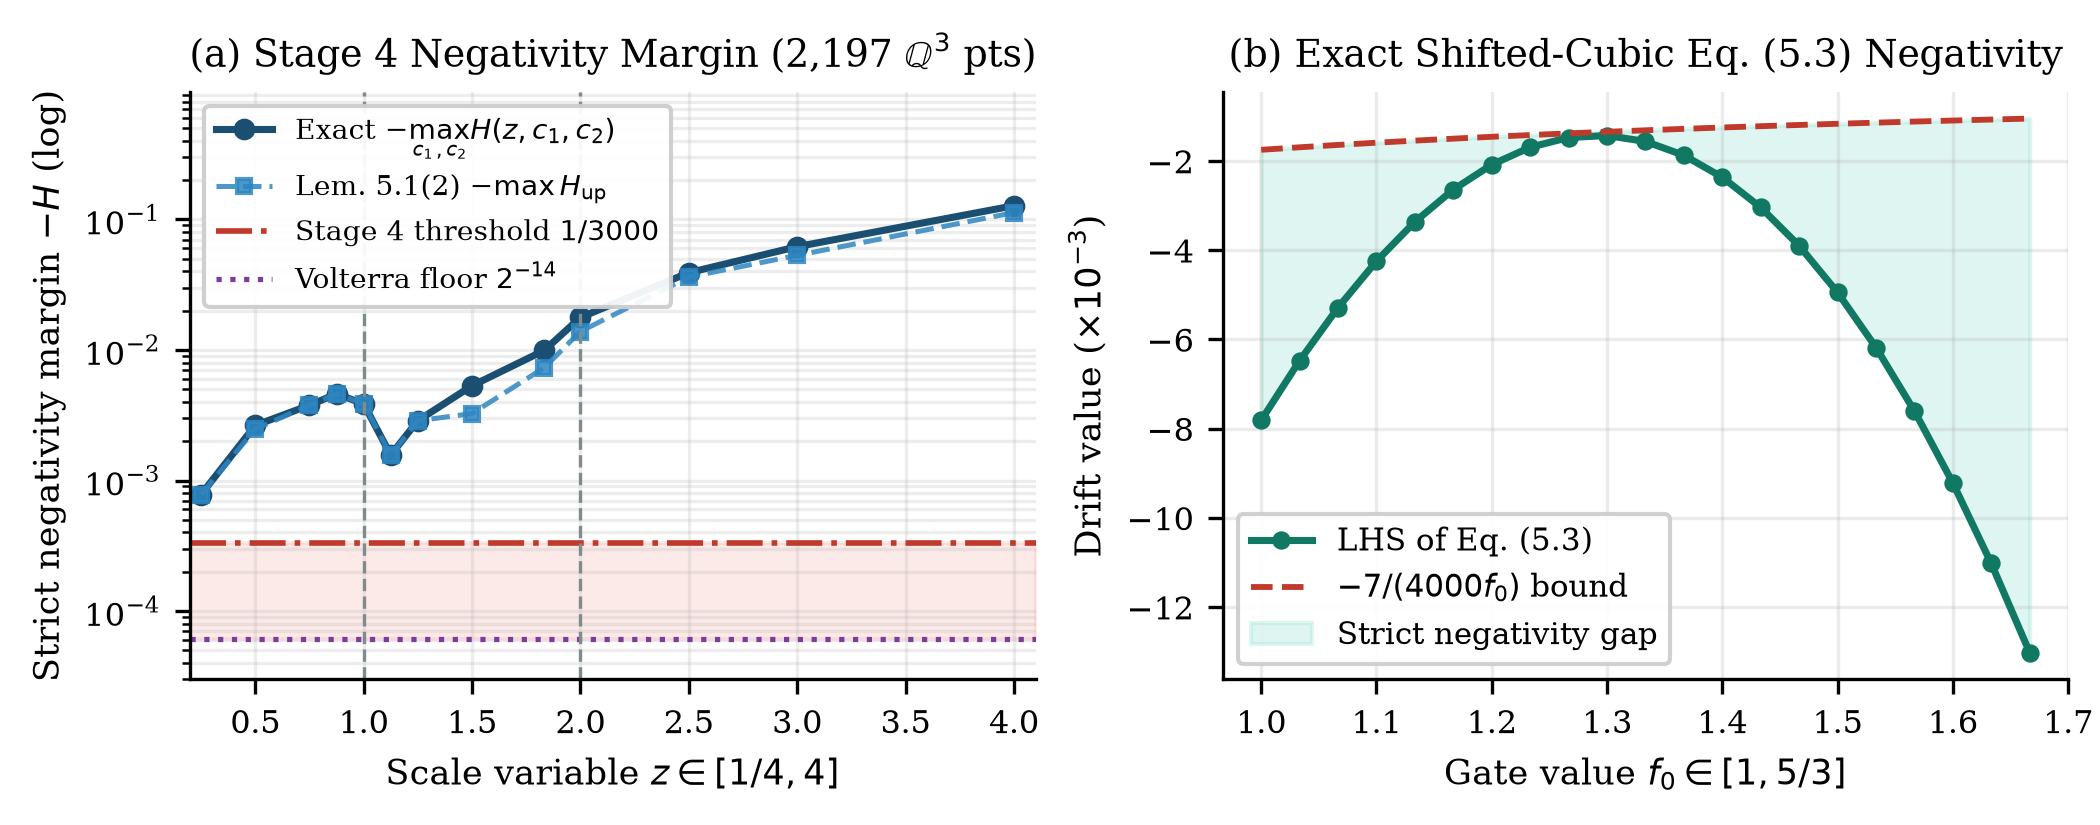
\includegraphics[width=\columnwidth]{figures/fig1_stage4_landscape_and_eq53.png}
\vspace{-1.4em}
\caption{\textbf{(a)}~Exact-$\QQ$ Stage~4 negativity margin $-\max_{c_1,c_2} H(z,c_1,c_2)$ across all $13^3=2{,}197$ grid points on $[1/4,4]^3$ (log scale), uniformly exceeding $1/3000$ (global tightest point $-1/1280$ at $(1/4,1/4,1/4)$) and separated by over an order of magnitude from the Volterra floor $2^{-14}$. \textbf{(b)}~Exact verification of the shifted-cubic drift bound Eq.~(5.3) on $f_0\in[1,5/3]$.}
\label{fig:stage4}
\end{figure}

\begin{figure}[t]
\centering
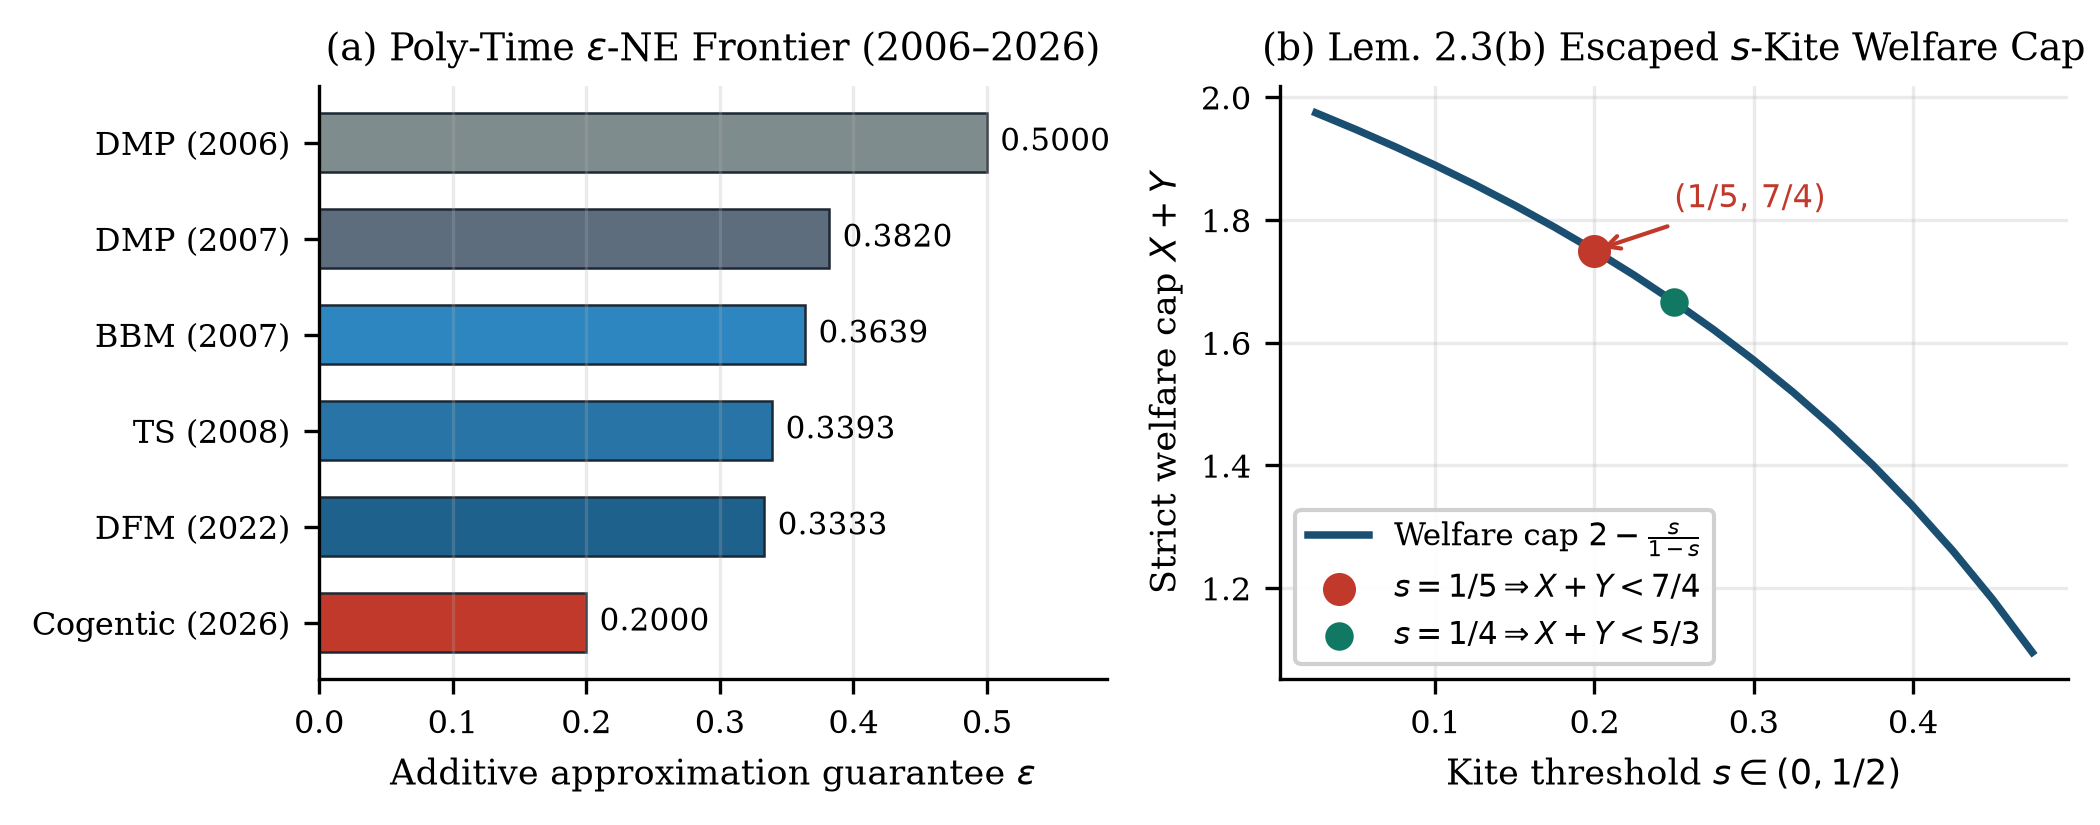
\includegraphics[width=\columnwidth]{figures/fig2_frontier_and_kite_cap.png}
\vspace{-1.4em}
\caption{\textbf{(a)}~Two-decade progression of polynomial-time additive $\varepsilon$-NE guarantees culminating at $1/5$~\cite{cogentic2026maximin}. \textbf{(b)}~Exact Lem.~2.3(b) strict welfare cap $2-s/(1-s)$ forced upon escaping the $s$-kite, highlighting $(1/5,7/4)$ and $(1/4,5/3)$.}
\label{fig:frontier}
\end{figure}

\section{Experiments, Certificate Atlas, and Red-Team Audit}\label{sec:exp}
All experiments were executed locally on Windows~11 (Python~3.12.6, Lean~4.35.0; 7-run means after warm-up).

\paragraph{1. 3D Exact-$\QQ$ Stage~4 Grid Sweep.}
Evaluating Eqs.~(\ref{eq:gate})--(\ref{eq:H}) over the $13^3 = 2{,}197$-point exact rational grid $z,c_1,c_2 \in \{\frac14,\frac12,\frac34,\frac78,1,\frac98,\frac54,\frac32,\frac{11}{6},2,\frac52,3,4\}$ confirms $H(z,c_1,c_2) \le -1/1280 \approx -7.813\times 10^{-4} \le -1/3000 < -2^{-14}$ at every single point (Fig.~\ref{fig:stage4}(a)), with the tightest slice at $z=1/4$ ($-1/1280$), followed by $z=9/8$ ($-481/307200 \approx -1.566\times 10^{-3}$) and deepening smoothly to $-19583/153600 \approx -0.1275$ at $z=4$. Every point also satisfies $H \le H_{\mathrm{up}}$ and $J \le J_{\mathrm{mid}}$.

\paragraph{2. Canonical 16-Certificate Atlas.}
Table~\ref{tab:atlas} records all 16 canonical witnesses spanning Modes~1--4, verified in $0.104$--$2.564\,\mathrm{ms}$ (Fig.~\ref{fig:atlas}(a)). Mode~1 includes a zero-slack tight $1/5$-kite row mix (\texttt{kite\_row\_mix\_tight\_1\_5}: $r_1=1/4$, $r_2=0$, $(4/5)r_1=1/5$, output regret $1/5$) and escaped welfare-cap certificates at $s=1/5$ ($3/2 < 7/4$, $a=3/2$) and $s=1/4$ ($6/5 < 5/3$, $a=5/3$). Mode~2 covers both \texttt{early\_halt} ($\max(v_R,v_C)\le 1/5$, including exact boundary $v_R=v_C=1/5$) and \texttt{anchored\_continue} (Row-oriented $v_R\ge v_C$, guaranteed floors $13/32 > 1/20$ and $43/160 > 1/20$) alongside exact denominator-$D$ simplex rounding (Fig.~\ref{fig:atlas}(b)). Mode~3 certifies 48 distinct exact rational probes across all three gate regimes plus adversarial corners. Mode~4 certifies end-to-end $1/5$-NE bimatrix profiles up to $5\times 5$, including a zero-slack $4\times 4$ profile with $r_1=r_2=1/5$ and an exact Nash equilibrium ($\rho=0$).

\begin{figure}[t]
\centering
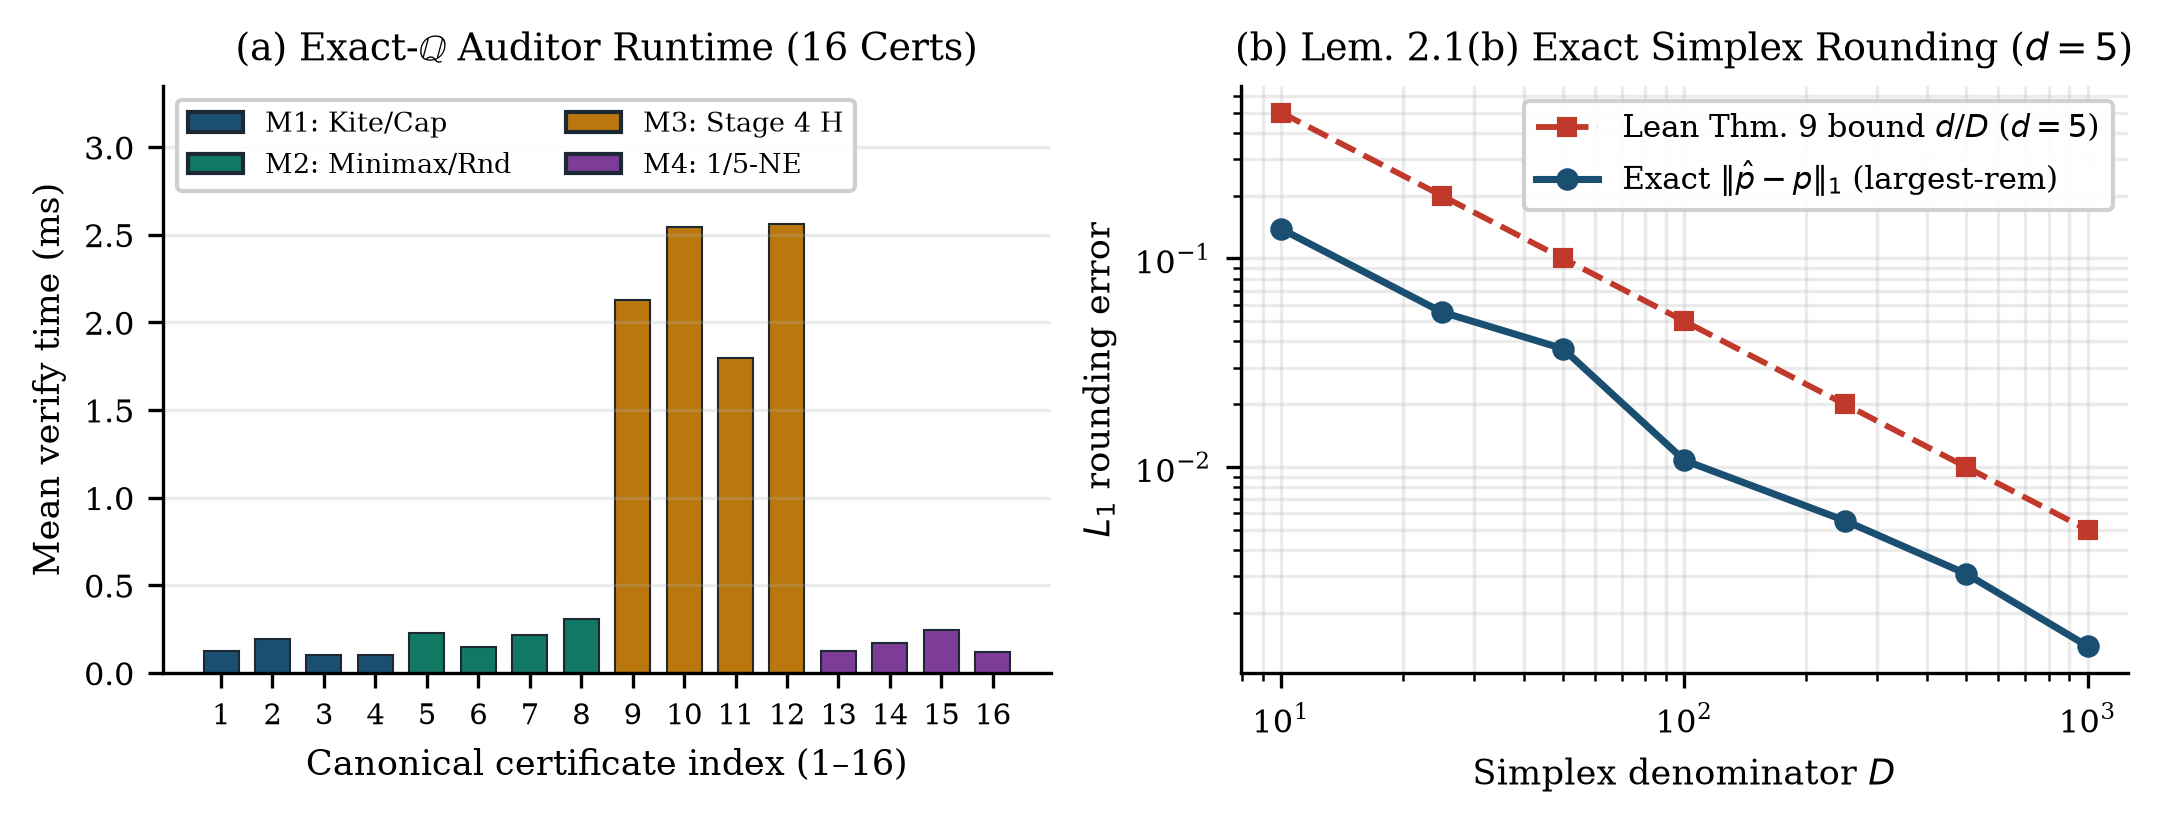
\includegraphics[width=\columnwidth]{figures/fig3_atlas_and_rounding.png}
\vspace{-1.4em}
\caption{\textbf{(a)}~Mean exact-$\QQ$ verification latency across all 16 canonical certificates ($0.104$--$2.564\,\mathrm{ms}$). \textbf{(b)}~Exact $L_1$ simplex rounding error $\|\hat{p}-p\|_1$ vs.\ the Lean Theorem~9 upper bound $d/D$ ($d=5$, $D\in[10,1000]$).}
\label{fig:atlas}
\end{figure}

\paragraph{3. Live Adversarial Forgery \& Integrity Gate.}
\texttt{tests/test\_suite.py} runs 64 pytest checks (all passing in $0.11\,\mathrm{s}$): all 16 canonical certificates, 3 raw-JSON IEEE-754/\texttt{NaN}/duplicate-key parser rejections, and 60 live adversarial forgery mutations spanning schema/parser bypasses (10), Mode~1 kite/dual tampering (14), Mode~2 saddle/rounding/anchor tampering (14), Mode~3 domain/regime/duplicate/margin tampering (12), and Mode~4 regret/stage/support tampering (10). \texttt{scripts/verify\_all.py} passes all 5 gates including a strict axiom whitelist and 40-file SHA-256 manifest.

\begin{table}[t]
\centering
\caption{Canonical 16-certificate \texttt{KITE-NASH-CERT-1.0} atlas (\texttt{results/exp1\_certificate\_atlas.json}; all 16 verified).}
\label{tab:atlas}
\scriptsize
\setlength{\tabcolsep}{2.4pt}
\resizebox{\columnwidth}{!}{%
\begin{tabular}{@{}l c l r@{}}
\toprule
Certificate ID & M & Exact Certified Witness Summary & ms \\
\midrule
\texttt{kite\_row\_mix\_tight\_1\_5} & M1 & $s{=}\frac15, r_1{=}\frac14, r_2{=}0$, tight mix $\rho'{=}\frac15$ & 0.128 \\
\texttt{kite\_col\_mix\_asymmetric\_3x3} & M1 & $s{=}\frac15, r_1{=}\frac{1}{10}, r_2{=}\frac{11}{50}$, col mix $\rho'{=}\frac15$ & 0.196 \\
\texttt{kite\_escape\_welfare\_7\_4\_cap} & M1 & $s{=}\frac15$, $u_R{+}u_C{=}\frac32<\frac74$, $\lambda^*{=}\frac35, a{=}\frac32$ & 0.104 \\
\texttt{kite\_escape\_general\_s1\_4} & M1 & $s{=}\frac14$, $u_R{+}u_C{=}\frac65<\frac53$, $\lambda^*{=}\frac58, a{=}\frac53$ & 0.104 \\
\texttt{minimax\_early\_halt\_diag\_1\_6} & M2 & $v_R{=}\frac16, v_C{=}\frac15\le\frac15$, halt $\rho{=}0$, $L_1{=}\frac{1}{28}$ & 0.228 \\
\texttt{minimax\_early\_halt\_boundary\_1\_5} & M2 & $v_R{=}v_C{=}\frac15\le\frac15$, halt $\rho{=}0$, $L_1{=}\frac{2}{165}$ & 0.151 \\
\texttt{minimax\_anchored\_continue\_rps} & M2 & $v_R{=}v_C{=}\frac12$, floor $\frac{13}{32}>\frac{1}{20}$, $L_1{=}0$ & 0.219 \\
\texttt{minimax\_anchored\_4x4\_tight} & M2 & $v_R{=}\frac25, v_C{=}\frac{3}{10}$, floor $\frac{43}{160}$, $L_1{=}\frac{7}{650}$ & 0.307 \\
\texttt{stage4\_low\_gate\_grid\_z\_le\_1} & M3 & 12 pts $z\le 1$, $\max H{=}{-}\frac{1}{1280}\le{-}\frac{1}{3000}$ & 2.128 \\
\texttt{stage4\_high\_gate\_mid\_1\_to\_2} & M3 & 12 pts $z\in(1,2]$, $\max H{=}{-}\frac{127}{25600}$ & 2.547 \\
\texttt{stage4\_high\_gate\_top\_2\_to\_4} & M3 & 10 pts $z\in(2,4]$, $\max H{=}{-}\frac{2229}{51200}$ & 1.799 \\
\texttt{stage4\_corners\_and\_kinks\_full} & M3 & 14 corner/kink pts, $\max H{=}{-}\frac{983}{153600}$ & 2.564 \\
\texttt{ne\_one\_fifth\_kite\_mix\_3x3} & M4 & $3{\times}3$ \texttt{stage2\_kite}, $\rho{=}\frac15$, supp $(1,2)$ & 0.124 \\
\texttt{ne\_one\_fifth\_4x4\_zero\_slack} & M4 & $4{\times}4$ zero-slack $r_1{=}r_2{=}\frac15$, $\mathrm{lcm}{=}5$ & 0.171 \\
\texttt{ne\_one\_fifth\_5x5\_anchored\_lp} & M4 & $5{\times}5$ \texttt{stage3\_anchored\_lp}, $\rho{=}\frac{1}{50}$, $\mathrm{lcm}{=}60$ & 0.243 \\
\texttt{ne\_exact\_equilibrium\_3x3\_rps} & M4 & $3{\times}3$ \texttt{exact\_ne}, $\rho{=}0$, supp $(3,3)$ & 0.119 \\
\bottomrule
\end{tabular}}
\end{table}

\section{Conclusion}\label{sec:conc}
We delivered an independent, zero-dependency, zero-floating-point verification stack for Google Research Cogentic's exact polynomial-time $1/5$-approximate Nash equilibrium algorithm~\cite{cogentic2026maximin}, combining 18 constructive Lean~4.35.0 theorems (zero \texttt{sorry}, zero \texttt{Classical.choice}), the 4-mode exact-$\QQ$ auditor \texttt{KITE-NASH-CERT-1.0}, 16 canonical certificates, a $2{,}197$-point exact rational confirmation of $H \le -1/3000 < -2^{-14}$, and 60/60 live adversarial forgery rejections.

\bibliographystyle{plain}
\bibliography{references}
\end{document}
